% Options for packages loaded elsewhere
\PassOptionsToPackage{unicode}{hyperref}
\PassOptionsToPackage{hyphens}{url}
%
\documentclass[
  letterpaper,
  ignorenonframetext,
  aspectratio=43,
  handout,
  12pt]{beamer}
\usepackage{pgfpages}
\setbeamertemplate{caption}[numbered]
\setbeamertemplate{caption label separator}{: }
\setbeamercolor{caption name}{fg=normal text.fg}
\beamertemplatenavigationsymbolsempty
% Prevent slide breaks in the middle of a paragraph
\widowpenalties 1 10000
\raggedbottom
\setbeamertemplate{part page}{
  \centering
  \begin{beamercolorbox}[sep=16pt,center]{part title}
    \usebeamerfont{part title}\insertpart\par
  \end{beamercolorbox}
}
\setbeamertemplate{section page}{
  \centering
  \begin{beamercolorbox}[sep=12pt,center]{part title}
    \usebeamerfont{section title}\insertsection\par
  \end{beamercolorbox}
}
\setbeamertemplate{subsection page}{
  \centering
  \begin{beamercolorbox}[sep=8pt,center]{part title}
    \usebeamerfont{subsection title}\insertsubsection\par
  \end{beamercolorbox}
}
\AtBeginPart{
  \frame{\partpage}
}
\AtBeginSection{
  \ifbibliography
  \else
    \frame{\sectionpage}
  \fi
}
\AtBeginSubsection{
  \frame{\subsectionpage}
}
\usepackage{lmodern}
\usepackage{amssymb,amsmath}
\usepackage{ifxetex,ifluatex}
\ifnum 0\ifxetex 1\fi\ifluatex 1\fi=0 % if pdftex
  \usepackage[T1]{fontenc}
  \usepackage[utf8]{inputenc}
  \usepackage{textcomp} % provide euro and other symbols
\else % if luatex or xetex
  \usepackage{unicode-math}
  \defaultfontfeatures{Scale=MatchLowercase}
  \defaultfontfeatures[\rmfamily]{Ligatures=TeX,Scale=1}
\fi
\usetheme[]{metropolis}
% Use upquote if available, for straight quotes in verbatim environments
\IfFileExists{upquote.sty}{\usepackage{upquote}}{}
\IfFileExists{microtype.sty}{% use microtype if available
  \usepackage[]{microtype}
  \UseMicrotypeSet[protrusion]{basicmath} % disable protrusion for tt fonts
}{}
\makeatletter
\@ifundefined{KOMAClassName}{% if non-KOMA class
  \IfFileExists{parskip.sty}{%
    \usepackage{parskip}
  }{% else
    \setlength{\parindent}{0pt}
    \setlength{\parskip}{6pt plus 2pt minus 1pt}}
}{% if KOMA class
  \KOMAoptions{parskip=half}}
\makeatother
\usepackage{xcolor}
\IfFileExists{xurl.sty}{\usepackage{xurl}}{} % add URL line breaks if available
\IfFileExists{bookmark.sty}{\usepackage{bookmark}}{\usepackage{hyperref}}
\hypersetup{
  hidelinks,
  pdfcreator={LaTeX via pandoc}}
\urlstyle{same} % disable monospaced font for URLs
\newif\ifbibliography
\usepackage{graphicx}
\makeatletter
\def\maxwidth{\ifdim\Gin@nat@width>\linewidth\linewidth\else\Gin@nat@width\fi}
\def\maxheight{\ifdim\Gin@nat@height>\textheight\textheight\else\Gin@nat@height\fi}
\makeatother
% Scale images if necessary, so that they will not overflow the page
% margins by default, and it is still possible to overwrite the defaults
% using explicit options in \includegraphics[width, height, ...]{}
\setkeys{Gin}{width=\maxwidth,height=\maxheight,keepaspectratio}
% Set default figure placement to htbp
\makeatletter
\def\fps@figure{htbp}
\makeatother
\setlength{\emergencystretch}{3em} % prevent overfull lines
\providecommand{\tightlist}{%
  \setlength{\itemsep}{0pt}\setlength{\parskip}{0pt}}
\setcounter{secnumdepth}{-\maxdimen} % remove section numbering
\usepackage{pgfpages}
\pgfpagesuselayout{2 on 1}
\providecommand{\tightlist}{%
\setlength{\itemsep}{0pt}\setlength{\parskip}{0pt}}
\makeatletter
\makeatother
\let\Oldincludegraphics\includegraphics
\renewcommand{\includegraphics}[2][]{\Oldincludegraphics[width=\textwidth,height=0.7\textheight,keepaspectratio]{#2}}
\ifluatex
  \usepackage{selnolig}  % disable illegal ligatures
\fi

\author{}
\date{}

\begin{document}

\begin{frame}{Mechanics of Materials}
\protect\hypertarget{mechanics-of-materials}{}
Lecture 19 - Discontinuity Functions

Dr.~Nicholas Smith

Wichita State University, Department of Aerospace Engineering

27 October, 2020
\end{frame}

\begin{frame}{schedule}
\protect\hypertarget{schedule}{}
\begin{itemize}
\tightlist
\item
  27 Oct - Beam Deflection (discontinuity functions), HW 8 Due, HW 7
  Self-Grade Due
\item
  29 Oct - Beam Deflection (superposition)
\item
  3 Nov - Statically Indeterminate Beams, HW 9 Due, HW 8 Self-Grade Due
\item
  5 Nov - Statically Indeterminate Beams
\end{itemize}
\end{frame}

\begin{frame}{outline}
\protect\hypertarget{outline}{}
\begin{itemize}
\tightlist
\item
  discontinuity functions
\item
  group problems
\end{itemize}
\end{frame}

\begin{frame}{discontinuity functions}
\protect\hypertarget{discontinuity-functions}{}
\begin{itemize}
\tightlist
\item
  Direct integration can be very cumbersome if multiple loads or
  boundary conditions are applied
\item
  Instead of using a piecewise function, we can use discontinuity
  functions
\end{itemize}
\end{frame}

\begin{frame}{Macaulay functions}
\protect\hypertarget{macaulay-functions}{}
\begin{itemize}
\tightlist
\item
  Macaulay functions can be used to describe various loading conditions,
  the general definition is
\end{itemize}

\[\langle x-a\rangle^n = \begin{cases}
  0 & \text{for } x < a\
  (x-a)^n & \text{for } x \ge a
\end{cases}
n \ge 0\]
\end{frame}

\begin{frame}{singularity functions}
\protect\hypertarget{singularity-functions}{}
\begin{itemize}
\tightlist
\item
  Singularity functions are used for concentrated forces and can be
  written
\end{itemize}

\[w = P\langle x-a\rangle^{-1} = \begin{cases}
  0 & \text{for } x\ne a\
  P & \text{for } x=a
\end{cases}\]
\end{frame}

\begin{frame}{discontinuity functions}
\protect\hypertarget{discontinuity-functions-1}{}
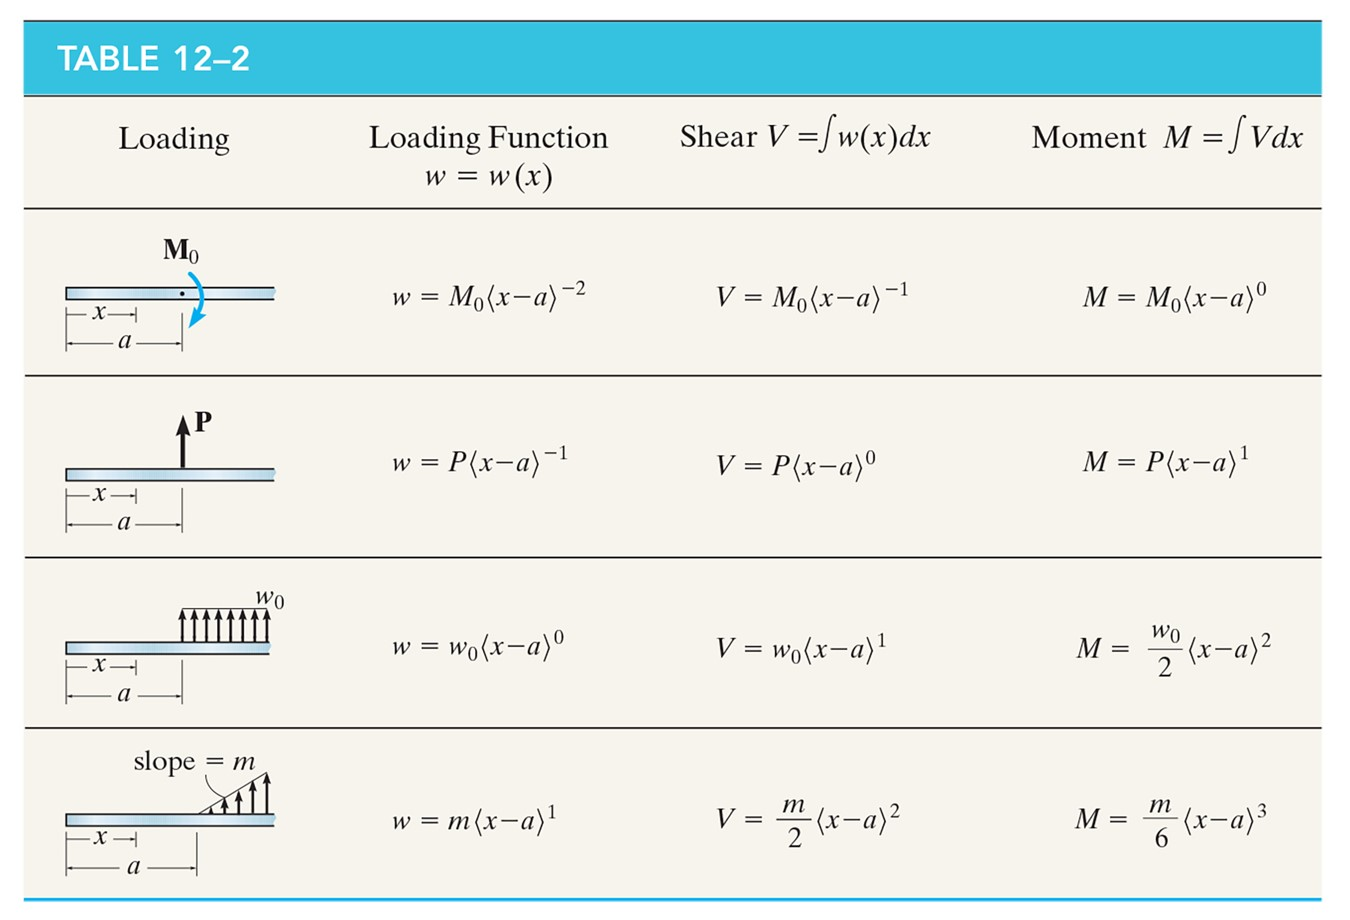
\includegraphics{../images/discontinuity.jpg}
\end{frame}

\begin{frame}{discontinuity functions}
\protect\hypertarget{discontinuity-functions-2}{}
\begin{enumerate}
\tightlist
\item
  We add these up for each loading case along our beam
\item
  We integrate as usual to find displacement from load, slope, or moment
\end{enumerate}
\end{frame}

\begin{frame}{integration}
\protect\hypertarget{integration}{}
\begin{itemize}
\tightlist
\item
  discontinuity functions follow special rules for integration
\item
  when \(n \ge 0\), they integrate like a normal polynomial
\item
  when \(n < 0\), they instead follow
  \[ \int \langle x-a \rangle ^n dx = \langle x - a \rangle ^{n+1} \]
\end{itemize}
\end{frame}

\begin{frame}{signs}
\protect\hypertarget{signs}{}
\begin{itemize}
\tightlist
\item
  we need to be careful to match the sign convention
\item
  loads are defined as positive when they act upward
\item
  moments are defined as positive when they act clockwise
\end{itemize}
\end{frame}

\begin{frame}{example 12.5}
\protect\hypertarget{example-12.5}{}
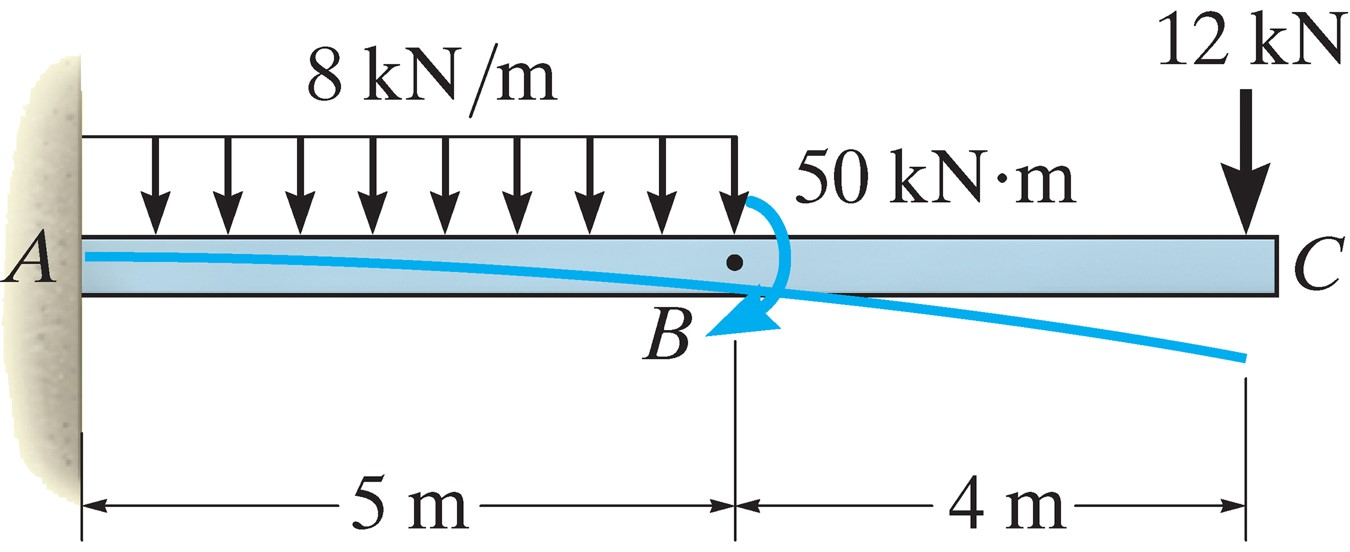
\includegraphics{../images/example-12-5.jpg}
\end{frame}

\begin{frame}{group one}
\protect\hypertarget{group-one}{}
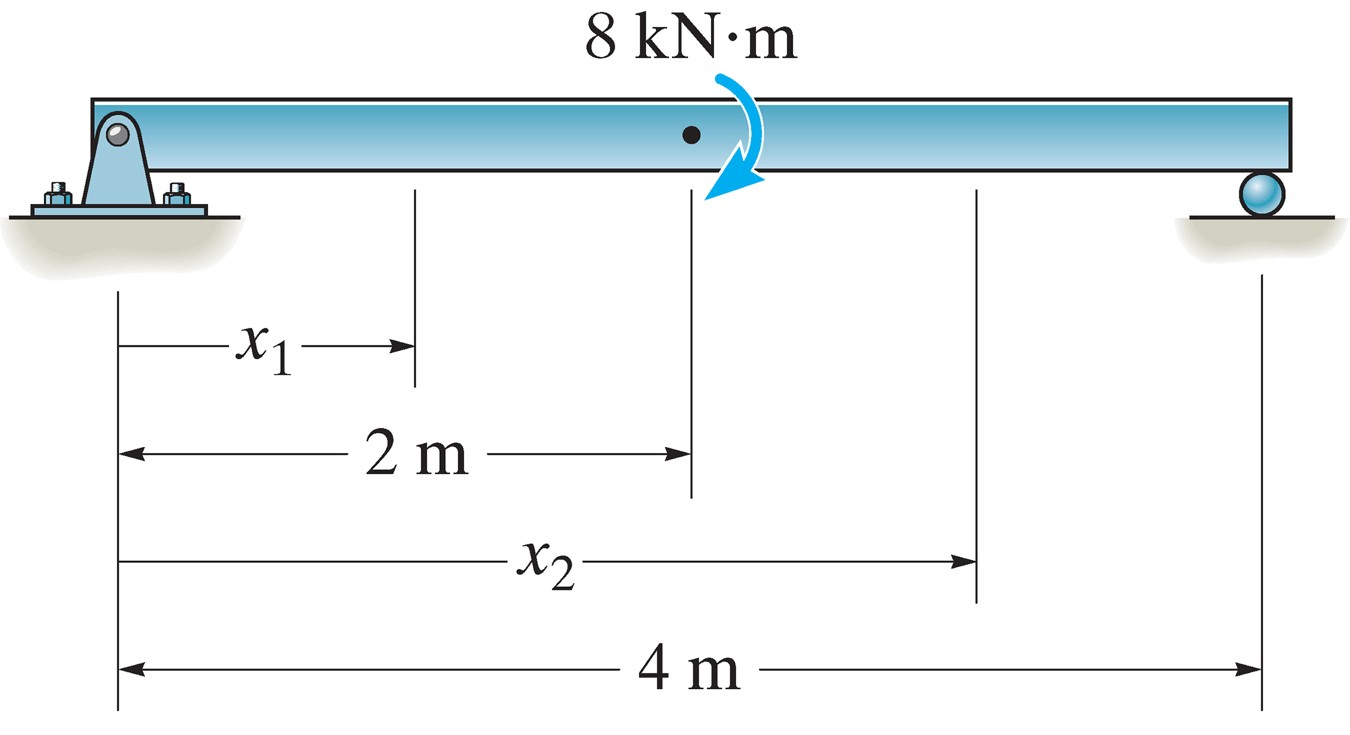
\includegraphics{../images/group-12-1.jpg}

Find the maximum deflection using either direct integration or
discontinuity functions.
\end{frame}

\begin{frame}{group two}
\protect\hypertarget{group-two}{}
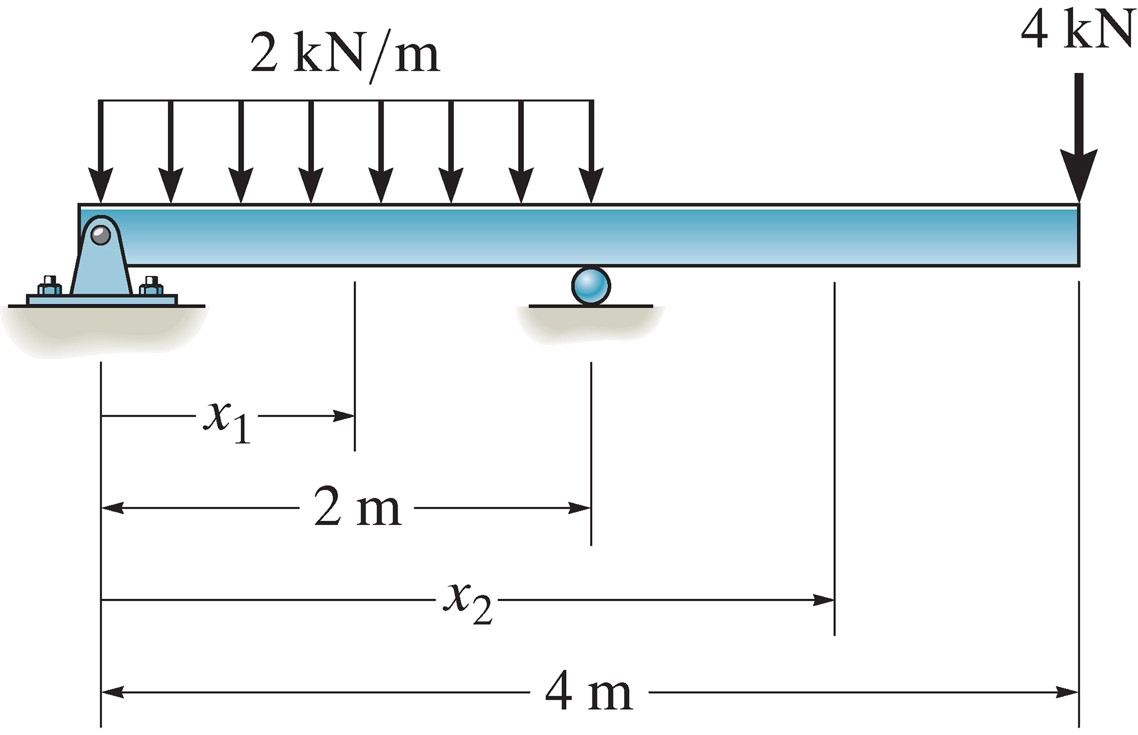
\includegraphics{../images/group-12-2.jpg}

Find the maximum deflection using either direct integration or
discontinuity functions.
\end{frame}

\begin{frame}{group three}
\protect\hypertarget{group-three}{}
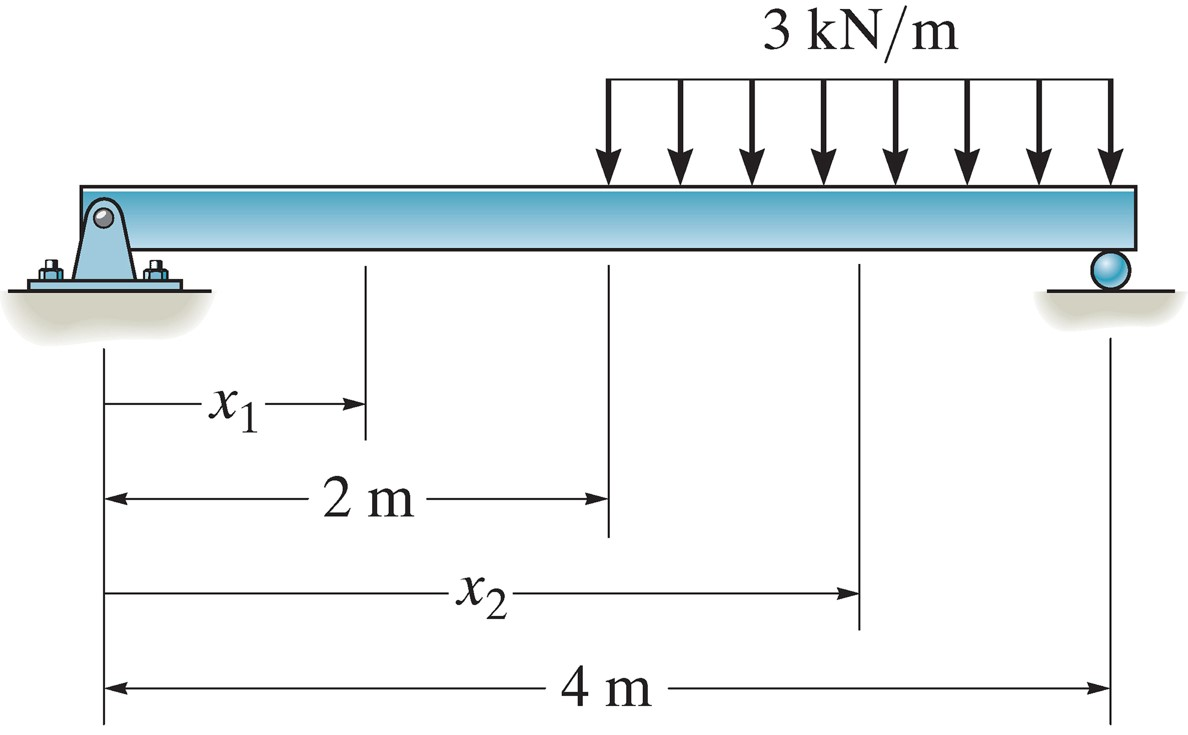
\includegraphics{../images/group-12-3.jpg}

Find the maximum deflection using either direct integration or
discontinuity functions.
\end{frame}

\end{document}
